\documentclass[12pt]{article}
\usepackage[margin=1in]{geometry}
\usepackage{amsmath,amssymb,amsthm,booktabs,graphicx,natbib,microtype}
\newtheorem{theorem}{Theorem}
\newtheorem{corollary}[theorem]{Corollary}
\newtheorem{proposition}[theorem]{Proposition}
\newtheorem{remark}[theorem]{Remark}
\newcommand{\R}{\mathbb{R}}
\title{A Finite-Anchor Barrier for Physical Scale Laws\\\large Bounded Smooth Continuations and a Five-Scale Envelope Audit}
\author{Prime Dynamics Theory Program}
\date{July 2026}

\begin{document}
\maketitle

\begin{abstract}
The recent finite-memory route produces increasingly complete support
certificates on five physical scales, but an all-level theorem requires
control as the scale tends to zero.  We place the available capacity,
exterior-concentration, fourth-volume, fourth-mode, and memory-depth data into
one aligned envelope ledger.  Descriptive power-law fits are unstable: the
median-capacity exponent is $-4.496$, while leave-one-out fits range from
$-5.836$ to $-2.621$; the worst fitted envelope misses an anchor by a factor
of $142$.  We then prove a finite-anchor asymptotic nonidentifiability
theorem.  Any finite collection of positive anchors admits a smooth positive
continuation with an arbitrary prescribed positive germ near zero.  A
bounded version preserves a known interval such as $0<f<1$ while producing
continuations with limits $0$, an arbitrary interior constant, or $1$.
Thus even exact finite anchors plus the natural capacity range cannot imply
an all-level law.  The negative fitted exponents of bounded ratios are also
necessarily pre-asymptotic.  An independent physical inequality, not
extrapolation, is the next required input.
\end{abstract}

\section{The five-scale question}
The fourth-mode factorization is
\[
 q_4=\frac{\nu_4}{\Lambda_{23}},\qquad
 \Lambda_{23}=q_2q_3,
\]
where $q_j=s_j/s_1$ and $\nu_4=q_2q_3q_4$.  RH-110 bounded the capacity
$\Lambda_{23}$, RH-111 refined the exterior-volume estimate by a physical
concentration factor, and RH-116 made memory depth an exact first-passage
optimization.  These are finite operator statements.  To close the route at
all later levels one would need scale-uniform bounds for the numerator,
denominator, and directional tail factors.

It is tempting to fit the five observed scales and extrapolate.  This paper
separates two logically different claims:
\begin{enumerate}
 \item a descriptive fit summarizes the finite archive;
 \item an asymptotic law constrains every sufficiently small scale.
\end{enumerate}
Exploratory summaries are useful \citep{Tukey1977}, but the first claim alone
cannot imply the second.

\section{Smooth finite-anchor extensions}
Let $0<\sigma_m<\cdots<\sigma_1$ be distinct anchors and $y_i>0$.  Let $g$
be any positive smooth function on a neighborhood $(0,a)$ of zero.

\begin{theorem}[Positive finite-anchor extension]\label{thm:positive}
There exists $f\in C^\infty((0,\sigma_1])$ such that
\[
 f(\sigma_i)=y_i\quad(1\leq i\leq m),
 \qquad f(\sigma)=g(\sigma)\quad\text{for all sufficiently small }\sigma,
\]
and $f(\sigma)>0$ everywhere.
\end{theorem}
\begin{proof}
Choose $0<a<b<\sigma_m$ and a smooth cutoff $\chi$ that is zero on
$(0,a]$ and one on $[b,\sigma_1]$; standard bump functions provide such a
cutoff \citep{Hirsch1976}.  Let $p$ be the polynomial satisfying
$p(\sigma_i)=\log y_i$.  Define
\[
 f(\sigma)=\exp\!\left(\chi(\sigma)p(\sigma)
 +(1-\chi(\sigma))\log g(\sigma)\right).
\]
The exponential is positive and smooth.  At every anchor $\chi=1$, while
near zero $\chi=0$, proving both identities.
\end{proof}

The positivity construction may ignore a known physical range.  The next
version does not.  For $A<B$, define the smooth diffeomorphism
\[
 T_{A,B}(y)=\log\frac{y-A}{B-y},\qquad A<y<B.
\]

\begin{theorem}[Bounded finite-anchor extension]\label{thm:bounded}
Suppose $A<y_i<B$ and $A<g(\sigma)<B$.  There is a smooth extension matching
all anchors and the germ as in Theorem~\ref{thm:positive}, with
$A<f(\sigma)<B$ at every scale.
\end{theorem}
\begin{proof}
Interpolate the transformed anchor values
$T_{A,B}(y_i)$ by a polynomial $p$.  Blend $p$ with
$T_{A,B}\circ g$ using the same cutoff, and apply $T_{A,B}^{-1}$.  The inverse
maps all real values strictly into $(A,B)$ and preserves both matching
regions.
\end{proof}

\begin{corollary}[Asymptotic nonidentifiability]\label{cor:barrier}
For any finite capacity anchors in $(0,1)$ there are smooth matching
continuations, all remaining in $(0,1)$, whose limits at zero are respectively
$0$, any chosen $c\in(0,1)$, and $1$.
\end{corollary}
\begin{proof}
Apply Theorem~\ref{thm:bounded} with germs $g_0(\sigma)=\sigma$,
$g_c(\sigma)=c$, and $g_1(\sigma)=1-\sigma$ after restricting to scales below
one.
\end{proof}

Thus a finite data set cannot determine even the limiting value, much less a
rate.  The result is conditional only on the absence of an additional
physical relation between scales; such a relation is exactly what the route
must now prove.

\begin{proposition}[Bounded negative-exponent obstruction]\label{prop:power}
If $0<f(\sigma)\leq B<\infty$ and
$f(\sigma)\sim c\sigma^\alpha$ as $\sigma\downarrow0$ for $c>0$, then
$\alpha\geq0$.
\end{proposition}
\begin{proof}
If $\alpha<0$, then $c\sigma^\alpha\to\infty$, contradicting the finite
upper bound and asymptotic equivalence.
\end{proof}

In particular, negative fitted exponents for $\Lambda_{23}$ or $q_4$, both
bounded by one, cannot persist as genuine zero-scale power laws.

\section{Aligned physical envelope audit}
We align RH-110 capacity and volume records, RH-111 concentration records,
and RH-116 depth records by scale, side, and time.  To avoid triple counting
threshold-dependent packet chains, the envelope table uses the primary
$10^{-8}$ chain.  It contains 120 physical updates.

\begin{table}[h]
\centering
\begin{tabular}{lrrrrr}
\toprule
$\sigma$ & records & median $\Lambda_{23}$ & median concentration & median $q_4$ & max depth\\
\midrule
$0.16$ & 8  & $5.51\,10^{-8}$ & $1.0000$ & $1.21\,10^{-8}$ & 3\\
$0.08$ & 12 & $2.28\,10^{-4}$ & $1.0030$ & $4.59\,10^{-5}$ & 5\\
$0.04$ & 22 & $7.76\,10^{-4}$ & $1.0090$ & $4.58\,10^{-4}$ & 6\\
$0.02$ & 34 & $2.63\,10^{-2}$ & $1.0001$ & $2.22\,10^{-2}$ & 4\\
$0.01$ & 44 & $3.00\,10^{-2}$ & $1.0656$ & $2.70\,10^{-2}$ & 4\\
\bottomrule
\end{tabular}
\caption{Primary-chain medians and the largest first-passage depth.}
\end{table}

Across all records, capacity ranges from $1.07\times10^{-11}$ to $0.388$,
and concentration ranges from $1$ to $2.330$.  The observed depth sequence
$3,5,6,4,4$ is bounded on the archive but not monotone in scale.

For each positive envelope statistic we fit
$y(\sigma)=C\sigma^\alpha$ by least squares in log coordinates.  These fits
are explicitly descriptive, not inferential or asymptotic.

\begin{table}[h]
\centering
\small
\begin{tabular}{lrrrr}
\toprule
metric & exponent & $R^2$ & max residual factor & leave-one-out exponent range\\
\midrule
capacity minimum & $-5.114$ & $0.728$ & $141.94$ & $[-6.561,-2.083]$\\
capacity median & $-4.496$ & $0.838$ & $13.61$ & $[-5.836,-2.621]$\\
concentration median & $-0.0179$ & $0.517$ & $1.028$ & $[-0.0249,-0.0009]$\\
fourth-mode median & $-5.109$ & $0.875$ & $11.94$ & $[-6.573,-3.320]$\\
\bottomrule
\end{tabular}
\caption{Finite-anchor power-law diagnostics.}
\end{table}

The apparently strong median trends coexist with order-of-magnitude
residuals and large leave-one-out drift.  Proposition~\ref{prop:power} gives
an even sharper warning: the negative exponents for bounded ratios must turn
over or saturate before the asymptotic regime.

The archived constructive audit applies Theorem~\ref{thm:bounded} to the five
median-capacity anchors.  Three continuations remain strictly in $(0,1)$ and
match every anchor to relative error below $1.7\times10^{-15}$.  At probe
scale $10^{-6}$ their values are $10^{-6}$, $1/2$, and $0.999999$.

\begin{figure}[h]
\centering
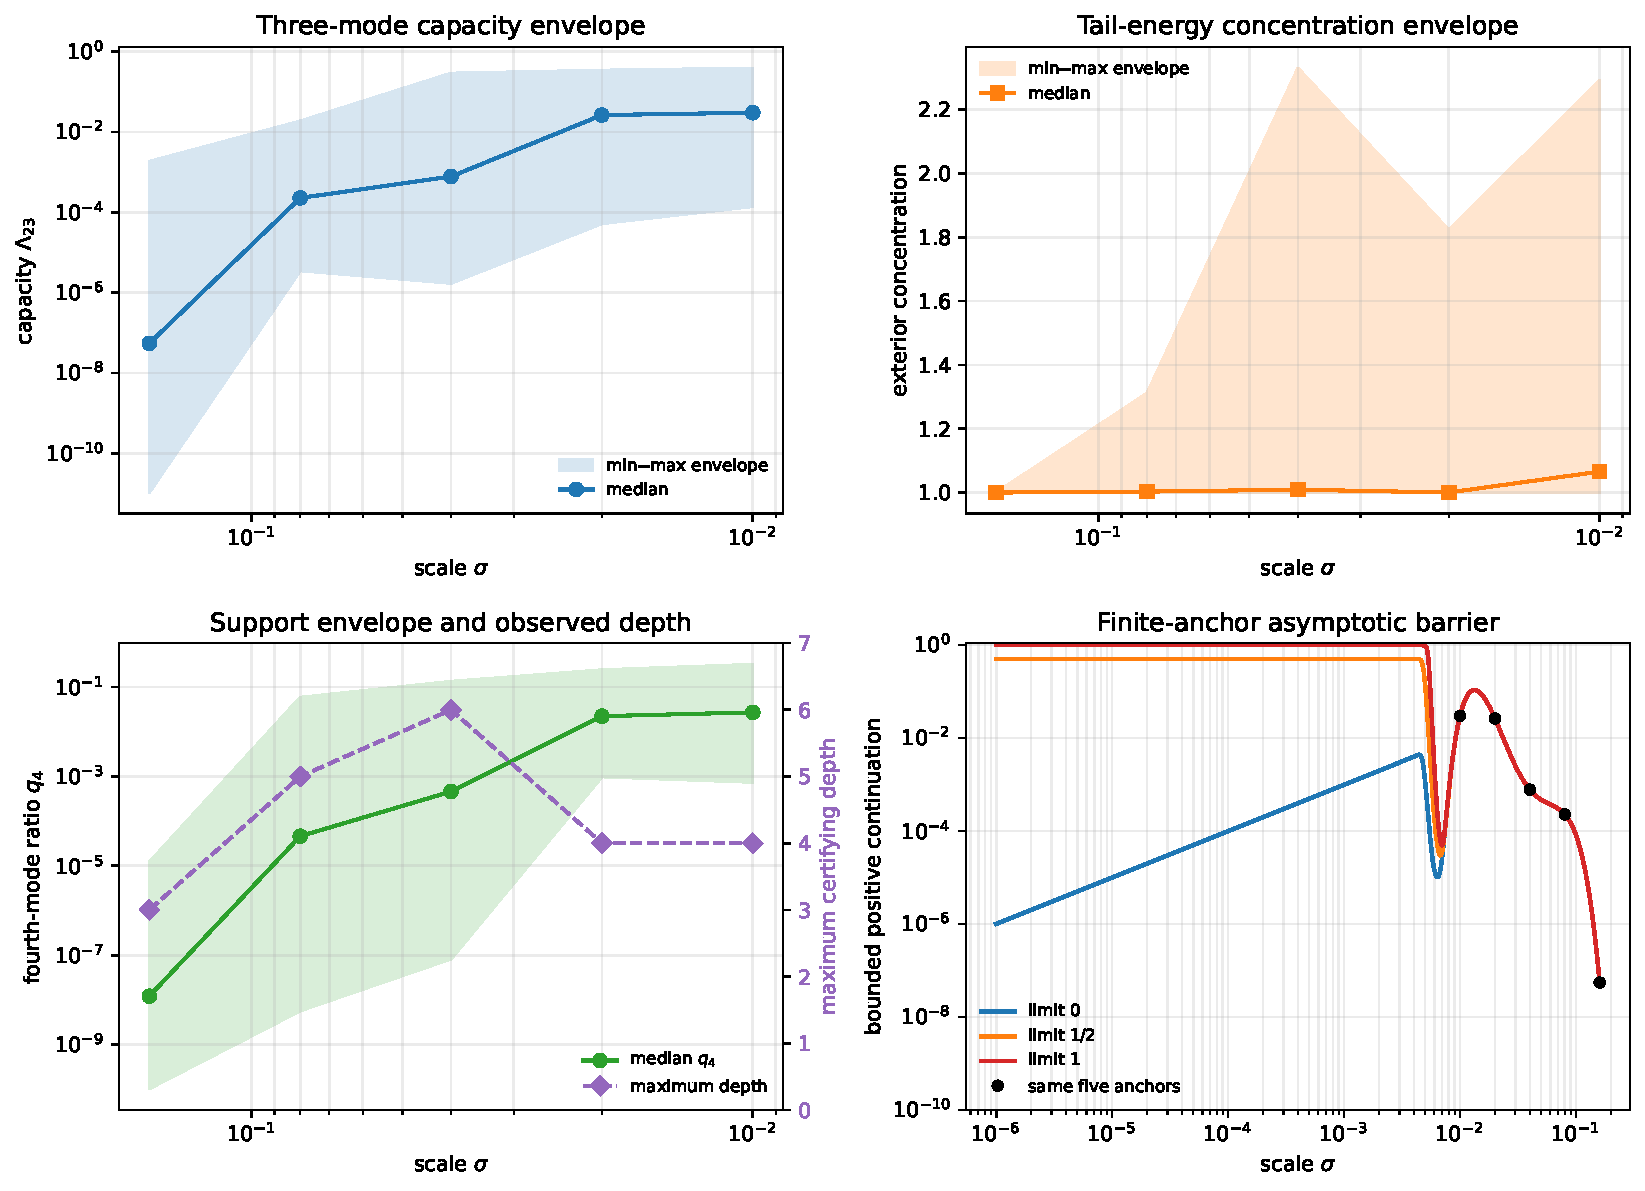
\includegraphics[width=\textwidth]{figures/finite_anchor_scale_law_barrier.pdf}
\caption{Physical envelopes, observed memory depth, and three bounded smooth
continuations through the same capacity anchors.}
\end{figure}

\section{Consequence and boundary}
RH-117 turns a vague caution about extrapolation into a precise obstruction.
The five-scale evidence is encouraging on the fine chain, but finite anchors
cannot supply the missing all-level hypothesis, even after imposing the
natural capacity range.  RH-118 should therefore state and prove a
conditional exterior-route theorem whose assumptions are explicit physical
inequalities, then identify the smallest unresolved all-level inputs.

This paper proves no all-level capacity, concentration, volume, directional,
or bounded-depth law.  It does not close uniform Stage A, construct a
Hilbert--Polya operator, identify zeta zeros, or prove the Riemann Hypothesis.

\bibliographystyle{plainnat}
\bibliography{references}
\end{document}
